\documentclass[11pt]{article}

%%%%%%%%%%%%%%%%%%%%%%%%%%%%%%%%%%%%%%%%%%%%%%%%%%%%%%%%%%%%%%%
%                      Customize Header                       %
%%%%%%%%%%%%%%%%%%%%%%%%%%%%%%%%%%%%%%%%%%%%%%%%%%%%%%%%%%%%%%%

\newcommand{\assessmentTitle}{
CheckIt Assessment
}
\newcommand{\assessmentVersion}{
Version 1770668285252
}
\newcommand{\assessmentInstructions}{
Do not use any unapproved aids while taking this assessment.
Read each question carefully and be sure to show all work
in the space provided.
}

%%%%%%%%%%%%%%%%%%%%%%%%%%%%%%%%%%%%%%%%%%%%%%%%%%%%%%%%%%%%%%%
%%%%%%%%%%%%%%%%%%%%%%%%%%%%%%%%%%%%%%%%%%%%%%%%%%%%%%%%%%%%%%%



\usepackage{amsfonts,amssymb,amsmath,amsthm}
\setcounter{MaxMatrixCols}{50}
\usepackage{hyperref}
\let\oldhref\href\renewcommand{\href}[2]{\oldhref{#1}{#2}\footnote{\url{#1}}}
\usepackage[margin=1in,tmargin=2in,headheight=84pt]{geometry}
\usepackage{enumerate}
\usepackage{graphicx}
\usepackage{fancyhdr}
\usepackage{lastpage}
\pagestyle{fancy}
\fancyhf{}
\rhead{Name: \underline{\hspace{2.5in}}\\ID: \underline{\hspace{2.5in}}

\vspace{2.5em}}
\chead{\vspace{2.5em}

\fbox{\fbox{\parbox{6in}{\centering\assessmentInstructions}}}}
\lhead{\assessmentTitle \hspace{2em} \assessmentVersion

\vspace{2.5em}}
\rfoot{Page \thepage\ of \pageref{LastPage}}
\setlength{\headheight}{80pt}
\renewcommand{\headrulewidth}{0pt}


\begin{document}

\begin{enumerate}

% 

\item %%%%% SpaTeXt Commands %%%%%
\providecommand{\stxKnowl}{}\renewcommand{\stxKnowl}[1]{#1}
\providecommand{\stxOuttro}{}\renewcommand{\stxOuttro}[1]{#1}
\providecommand{\stxTitle}{}\renewcommand{\stxTitle}[1]{#1}
% Comment next line to show outtros
\renewcommand{\stxOuttro}[1]{}
%%%%%%%%%%%%%%%%%%%%%%%%%%%%
\stxKnowl{
Evaluate the function \(f(x) = 4 \, x^{2} + 4 \, x + 6\).

\begin{enumerate}
\item
\stxKnowl{
Find \(f(7)\).

\stxOuttro{
SOLUTION

\(4(7)^2 + 4(7) + 6\)

\(\boxed{f(7) = 230}\)

}
}

\item
\stxKnowl{
Find \(f(-x)\).

\stxOuttro{
SOLUTION

\(4(-x)^2 + 4(-x) + 6\)

\(\boxed{f(-x) = 4 \, x^{2} - 4 \, x + 6}\)

}
}

\item
\stxKnowl{
Find \(f(x + a)\).

\stxOuttro{
SOLUTION

\(4(x+a)^2 + 4(x+a) + 6\)

\(\boxed{f(x + a) = 4 \, a^{2} + 8 \, a x + 4 \, x^{2} + 4 \, a + 4 \, x + 6}\)

}
}

\end{enumerate}
}

\newpage

% 

\item %%%%% SpaTeXt Commands %%%%%
\providecommand{\stxKnowl}{}\renewcommand{\stxKnowl}[1]{#1}
\providecommand{\stxOuttro}{}\renewcommand{\stxOuttro}[1]{#1}
\providecommand{\stxTitle}{}\renewcommand{\stxTitle}[1]{#1}
% Comment next line to show outtros
\renewcommand{\stxOuttro}[1]{}
%%%%%%%%%%%%%%%%%%%%%%%%%%%%
\stxKnowl{
 Determine the number and type of solutions for the following equation: 

 \(-x^{2} - 4 \, x - 1 = -2 \, x\) 

\stxOuttro{
SOLUTION

 \(-1x^2 + (-2)x + -1 = 0\) 

 \(\Delta = (-2)^2 - 4(-1)(-1)\) 

 \(\Delta = 0\) 

 \(\boxed{\text{ one solutions, repeated real root }}\) 

}
}

\newpage

% 

\item %%%%% SpaTeXt Commands %%%%%
\providecommand{\stxKnowl}{}\renewcommand{\stxKnowl}[1]{#1}
\providecommand{\stxOuttro}{}\renewcommand{\stxOuttro}[1]{#1}
\providecommand{\stxTitle}{}\renewcommand{\stxTitle}[1]{#1}
% Comment next line to show outtros
\renewcommand{\stxOuttro}[1]{}
%%%%%%%%%%%%%%%%%%%%%%%%%%%%
\stxKnowl{
Solve for all solutions. Identify any extraneous solutions.

 \(x^{2} - 6 \, x + 12 = 0\) 

\stxOuttro{
SOLUTION

 \(x = \frac{-(-6) \pm \sqrt{(-6)^2 - 4(1)(12)}}{2(1)}\) 

 \(= \frac{6 \pm \sqrt{36 - 48}}{2}\) 

 \(= \frac{6 \pm \sqrt{-12}}{2}\) 

 \(= \frac{6 \pm 2i\sqrt{3}}{2}\) 

 \(= \frac{2(3 \pm i\sqrt{3})}{2}\) 

 \(\boxed{x = 3 \pm i\sqrt{3}}\) 

 (No extraneous solutions) 

}
}

\newpage

% 

\item %%%%% SpaTeXt Commands %%%%%
\providecommand{\stxKnowl}{}\renewcommand{\stxKnowl}[1]{#1}
\providecommand{\stxOuttro}{}\renewcommand{\stxOuttro}[1]{#1}
\providecommand{\stxTitle}{}\renewcommand{\stxTitle}[1]{#1}
% Comment next line to show outtros
\renewcommand{\stxOuttro}[1]{}
%%%%%%%%%%%%%%%%%%%%%%%%%%%%
\stxKnowl{
Solve for all solutions. Identify any extraneous solutions.

 \(\sqrt{x + 73} + 1 = 9\) 

\stxOuttro{
SOLUTION

 \(\sqrt{x + 73} = 8\) 

 \(x + 73 = 64\) 

 \(x = 64 - 73\) 

 \(\boxed{x = -9}\) 

 (No extraneous solutions) 

}
}

\newpage

% 

\item %%%%% SpaTeXt Commands %%%%%
\providecommand{\stxKnowl}{}\renewcommand{\stxKnowl}[1]{#1}
\providecommand{\stxOuttro}{}\renewcommand{\stxOuttro}[1]{#1}
\providecommand{\stxTitle}{}\renewcommand{\stxTitle}[1]{#1}
% Comment next line to show outtros
\renewcommand{\stxOuttro}[1]{}
%%%%%%%%%%%%%%%%%%%%%%%%%%%%
\stxKnowl{
 Solve for all solutions. Identify any extraneous solutions. 

 \(\displaystyle \frac{x}{x + 1} + \frac{3}{(x + 1)(x + 4)} = \frac{-3}{x + 4}\) 

\stxOuttro{
SOLUTION

 \(x(x + 4) + 3 = -3(x + 1)\) 

 \(x^{2} + 7 \, x + 6 = 0\) 

 \((x + 1)(x + 6) = 0\) 

 \(x = -6, \quad x = -1\) 

 \(x = -1 \implies \text{Extraneous}\) 

 \(\boxed{x = -6}\) 

}
}

\newpage

% 

\item %%%%% SpaTeXt Commands %%%%%
\providecommand{\stxKnowl}{}\renewcommand{\stxKnowl}[1]{#1}
\providecommand{\stxOuttro}{}\renewcommand{\stxOuttro}[1]{#1}
\providecommand{\stxTitle}{}\renewcommand{\stxTitle}[1]{#1}
% Comment next line to show outtros
\renewcommand{\stxOuttro}[1]{}
%%%%%%%%%%%%%%%%%%%%%%%%%%%%
\stxKnowl{
 Given that the function is one-to-one, find the inverse function \(f^{-1}(x)\). 

 \(f(x) = \sqrt[3]{x - 2} - 3\) 

\stxOuttro{
SOLUTION

 \(y = f(x) = \sqrt[3]{x - 2} - 3\) 

 \(x = \sqrt[3]{y - 2} - 3\) 

 \(x + 3 = \sqrt[3]{y - 2}\) 

 \((x + 3)^3 = y - 2\) 

 \(y = (x + 3)^3 + 2\) 

 \(\boxed{ f^{-1}(x) = (x + 3)^3 + 2 }\) 

  

 \(= (x + 3)(x^2 + 6x + 9) + 2\) 

 \(\boxed{ f^{-1}(x) = x^{3} + 9 \, x^{2} + 27 \, x + 29 }\) 

}
}

\newpage

% 

\item %%%%% SpaTeXt Commands %%%%%
\providecommand{\stxKnowl}{}\renewcommand{\stxKnowl}[1]{#1}
\providecommand{\stxOuttro}{}\renewcommand{\stxOuttro}[1]{#1}
\providecommand{\stxTitle}{}\renewcommand{\stxTitle}[1]{#1}
% Comment next line to show outtros
\renewcommand{\stxOuttro}[1]{}
%%%%%%%%%%%%%%%%%%%%%%%%%%%%
\stxKnowl{
Suppose a rocket carrying fireworks is launched from a hill 45 feet above a lake. The rocket's height \(h\) (in feet) above the lake at time \(t\) (in seconds) is given by

 \(h(t) = -16t^2 + 96t + 45\) 

\begin{enumerate}
\item
\stxKnowl{
When will the rocket reach its maximum height?

\stxOuttro{
SOLUTION

 \(t = \frac{-96}{2(-16)} = \frac{-96}{-32}\) 

 \(\boxed{t = 3 \text{ sec}}\) 

}
}

\item
\stxKnowl{
What is the maximum height the rocket will reach?

\stxOuttro{
SOLUTION

 \(h(3) = -16(3)^2 + 96(3) + 45\) 

 \(= -144 + 288 + 45\) 

 \(\boxed{h = 189 \text{ ft}}\) 

}
}

\item
\stxKnowl{
Interpret your results for the previous two questions in one or more complete sentences, including appropriate units.

\stxOuttro{
SOLUTION

The rocket will reach a maximum height of 189 ft 3 seconds after launch.

}
}

\end{enumerate}
}

\newpage

% 

\item %%%%% SpaTeXt Commands %%%%%
\providecommand{\stxKnowl}{}\renewcommand{\stxKnowl}[1]{#1}
\providecommand{\stxOuttro}{}\renewcommand{\stxOuttro}[1]{#1}
\providecommand{\stxTitle}{}\renewcommand{\stxTitle}[1]{#1}
% Comment next line to show outtros
\renewcommand{\stxOuttro}[1]{}
%%%%%%%%%%%%%%%%%%%%%%%%%%%%
\stxKnowl{
 Given \(f(x) = -2 \, x\) and \(g(x) = 2 \, x^{2} - 1\), find the following: 

\begin{enumerate}
\item
\stxKnowl{
\((f \circ g)(x)\)

\stxOuttro{
SOLUTION

 \(f(g(x)) = -2(2 \, x^{2} - 1)\) 

 \(\boxed{ -4 \, x^{2} + 2 }\) 

ERROR 1: \(g(f(x))\)

 \(= 2(-2 \, x)^2 - 1\) 

 \(= 2(4 \, x^{2}) - 1\) 

 \(\boxed{ 8 \, x^{2} - 1 }\) 

ERROR 2: \(f(x) \cdot g(x)\)

 \(= (-2 \, x)(2 \, x^{2} - 1)\) 

 \(\boxed{ -4 \, x^{3} + 2 \, x }\) 

}
}

\item
\stxKnowl{
\((f \circ f)(x)\)

\stxOuttro{
SOLUTION

 \(f(f(x)) = -2(-2 \, x)\) 

 \(\boxed{ 4 \, x }\) 

}
}

\end{enumerate}
}

\newpage

% 

\item %%%%% SpaTeXt Commands %%%%%
\providecommand{\stxKnowl}{}\renewcommand{\stxKnowl}[1]{#1}
\providecommand{\stxOuttro}{}\renewcommand{\stxOuttro}[1]{#1}
\providecommand{\stxTitle}{}\renewcommand{\stxTitle}[1]{#1}
% Comment next line to show outtros
\renewcommand{\stxOuttro}[1]{}
%%%%%%%%%%%%%%%%%%%%%%%%%%%%
\stxKnowl{
 Evaluate the difference quotient, \(\displaystyle{ \frac{f(x+h)-f(x)}{h}}\) , for \(f(x) = 6 \, x^{2} + 1\). 

\stxOuttro{
SOLUTION

 \(f(x+h) = 6(x+h)^2 + 1\) 

 \(= 6(x^2 + 2xh + h^2) + 1\) 

 \(= 6 \, h^{2} + 12 \, h x + 6 \, x^{2} + 1\) 

 \(\displaystyle{\frac{f(x+h)-f(x)}{h} = \frac{ (6 \, h^{2} + 12 \, h x + 6 \, x^{2} + 1) - (6 \, x^{2} + 1) }{h}}\) 

 \(=\displaystyle{ \frac{ 6 \, h^{2} + 12 \, h x }{h}}\) 

 \(= \displaystyle{ \frac{ h(6 \, h + 12 \, x) }{h}}\) 

 \(\boxed{ 6 \, h + 12 \, x }\) 

}
}

\newpage

% 

\item %%%%% SpaTeXt Commands %%%%%
\providecommand{\stxKnowl}{}\renewcommand{\stxKnowl}[1]{#1}
\providecommand{\stxOuttro}{}\renewcommand{\stxOuttro}[1]{#1}
\providecommand{\stxTitle}{}\renewcommand{\stxTitle}[1]{#1}
% Comment next line to show outtros
\renewcommand{\stxOuttro}[1]{}
%%%%%%%%%%%%%%%%%%%%%%%%%%%%
\stxKnowl{
 Find each of the properties below for the given function: 

 \(f(x) = -\frac{1}{4}(x - 2)^2 +1\) 

\begin{itemize}
\item
Vertex

\item
Axis of Symmetry

\item
\(x\)-intercepts

\item
\(y\)-intercept

\item
Domain

\item
Range

\end{itemize}
\stxOuttro{
SOLUTION

 \(\textbf{Direction: } \text{Opens Down}\) 

 \(\textbf{Vertex: } (2, 1)\) 

 \(\textbf{Axis of Symmetry: } x = 2\) 

 \(\textbf{x-intercepts:}\) 

 \(-\frac{1}{4}(x - 2)^2 +1 = 0\) 

 \((x - 2)^2 = 4\) 

 \(x = 2 \pm 2\) 

 \(\boxed{ 0, 4 }\) 

 \(\textbf{y-intercept:}\) 

 \(= -\frac{1}{4}(0 - 2)^2 +1\) 

 \(= -\frac{1}{4}(4) +1\) 

 \(= -1 +1\) 

 \(\boxed{ 0 }\) 

 \(\textbf{Domain: } (-\infty, \infty)\) 

 \(\textbf{Range: } (-\infty, 1]\) 

}
}

\newpage

% 

\item %%%%% SpaTeXt Commands %%%%%
\providecommand{\stxKnowl}{}\renewcommand{\stxKnowl}[1]{#1}
\providecommand{\stxOuttro}{}\renewcommand{\stxOuttro}[1]{#1}
\providecommand{\stxTitle}{}\renewcommand{\stxTitle}[1]{#1}
% Comment next line to show outtros
\renewcommand{\stxOuttro}[1]{}
%%%%%%%%%%%%%%%%%%%%%%%%%%%%
\stxKnowl{
 A quadratic function has the characteristics given below. Use the axis of symmetry to generate two additional points, then use all five points to graph the function. 

\begin{itemize}
\item
\(\text{Vertex: } (-4, 9)\)

\item
\(x\text{-intercept: } -7\)

\item
\(y\text{-intercept: } -7\)

\end{itemize}
 \begin{tikzpicture}[scale=0.35] \draw[step=1cm, gray!40, very thin] (-10,-10) grid (10,10); \draw[thick, <->] (-10.5,0) -- (10.5,0); \draw[thick, <->] (0,-10.5) -- (0,10.5); \end{tikzpicture} 

\stxOuttro{
SOLUTION

 \begin{multicols}{2}  

\begin{itemize}
\item
\(\text{Vertex: } (-4, 9)\)

\item
\(y\text{-intercept: } (0, -7)\)

\item
\(\text{Reflected } y\text{-int: } (-8, -7)\)

\item
\(\text{Given Root: } (-7, 0)\)

\item
\(\text{Reflected Root: } (-1, 0)\)

\end{itemize}
 \columnbreak  

 \begin{tikzpicture}[scale=0.35] \draw[step=1cm, gray!40, very thin] (-10,-10) grid (10,10); \draw[thick, <->] (-10.5,0) -- (10.5,0); \draw[thick, <->] (0,-10.5) -- (0,10.5); \clip (-10,-10) rectangle (10,10); \draw[line width=1.5pt, blue!80!black, samples=100, domain=-10:10, <->] plot (\x, {-1.0*(\x - -4)^2 + 9}); \fill[blue] (-4,9) circle (7pt); \fill[blue] (-7,0) circle (7pt); \fill[blue] (-1,0) circle (7pt); \fill[blue] (0,-7) circle (7pt); \fill[blue] (-8,-7) circle (7pt); \end{tikzpicture} 

 \end{multicols} 

}
}

\newpage

% 

\item %%%%% SpaTeXt Commands %%%%%
\providecommand{\stxKnowl}{}\renewcommand{\stxKnowl}[1]{#1}
\providecommand{\stxOuttro}{}\renewcommand{\stxOuttro}[1]{#1}
\providecommand{\stxTitle}{}\renewcommand{\stxTitle}[1]{#1}
% Comment next line to show outtros
\renewcommand{\stxOuttro}[1]{}
%%%%%%%%%%%%%%%%%%%%%%%%%%%%
\stxKnowl{
 Use the table to identify the transformations described by \(g(x) = -2f(x) + 1\). Circle the option that applies and fill in the blanks as appropriate to describe the transformations of the given function. If one does not apply, you may leave it blank. Then apply these transformations to the graph of the function shown below. 

 \(\renewcommand{\arraystretch}{3} \begin{array}{|l|l|} \hline \textbf{Horizontal Transformations} & \textbf{Vertical Transformations} \\ \hline \text{Reflection: YES or NO} & \text{Reflection: YES or NO} \\ \hline \text{Dilation: \underline{\hspace{2cm}} times as wide} & \text{Dilation: \underline{\hspace{2cm}} times as tall} \\ \hline \text{Translation: \underline{\hspace{2cm}} units LEFT or RIGHT} & \text{Translation: \underline{\hspace{2cm}} units UP or DOWN} \\ \hline \end{array}\) 

 \noindent\makebox[\textwidth][c]{ \begin{minipage}{0.48\textwidth} \centering \begin{tikzpicture}[scale=0.39] \draw[step=1cm, gray!40, very thin] (-10,-10) grid (10,10); \draw[thick, <->] (-10.5,0) -- (10.5,0); \draw[thick, <->] (0,-10.5) -- (0,10.5); \draw[line width=1.5pt, black] (-2,1) -- (-1,2) -- (0,0) -- (1,4) -- (3,4);\fill[black] (-2,1) circle (5pt); \fill[black] (-1,2) circle (5pt); \fill[black] (0,0) circle (5pt); \fill[black] (1,4) circle (5pt); \fill[black] (3,4) circle (5pt); \end{tikzpicture} \end{minipage} \hfill \begin{minipage}{0.48\textwidth} \centering \begin{tikzpicture}[scale=0.39] \draw[step=1cm, gray!40, very thin] (-10,-10) grid (10,10); \draw[thick, <->] (-10.5,0) -- (10.5,0); \draw[thick, <->] (0,-10.5) -- (0,10.5); \end{tikzpicture} \end{minipage} } 

\stxOuttro{
SOLUTION



\begin{itemize}
\item
 \(\textbf{Horizontal: } \text{Reflection: NO, Dilation: 1, Shift: 0 units NONE.}\) 

\item
 \(\textbf{Vertical: } \text{Reflection: YES, Dilation: 2, Shift: 1 units UP.}\) 

\end{itemize}


 \begin{tikzpicture}[scale=0.39] \draw[step=1cm, gray!40, very thin] (-10,-10) grid (10,10); \draw[thick, <->] (-10.5,0) -- (10.5,0); \draw[thick, <->] (0,-10.5) -- (0,10.5); \draw[line width=1.5pt, blue] (-2,-1) -- (-1,-3) -- (0,1) -- (1,-7) -- (3,-7);\fill[blue] (-2,-1) circle (5pt); \fill[blue] (-1,-3) circle (5pt); \fill[blue] (0,1) circle (5pt); \fill[blue] (1,-7) circle (5pt); \fill[blue] (3,-7) circle (5pt); \end{tikzpicture} 

}
}

\newpage

% 

\end{enumerate}

\end{document}